\section[Content-based filtering]{Content-based filtering}
\begin{frame}[allowframebreaks, fragile]
	\frametitle{Content-based filtering}
    	Recommender systems are active information filtering systems that personalize the information coming to a user based on his interests, relevance of the information, etc. 
        \begin{figure}
            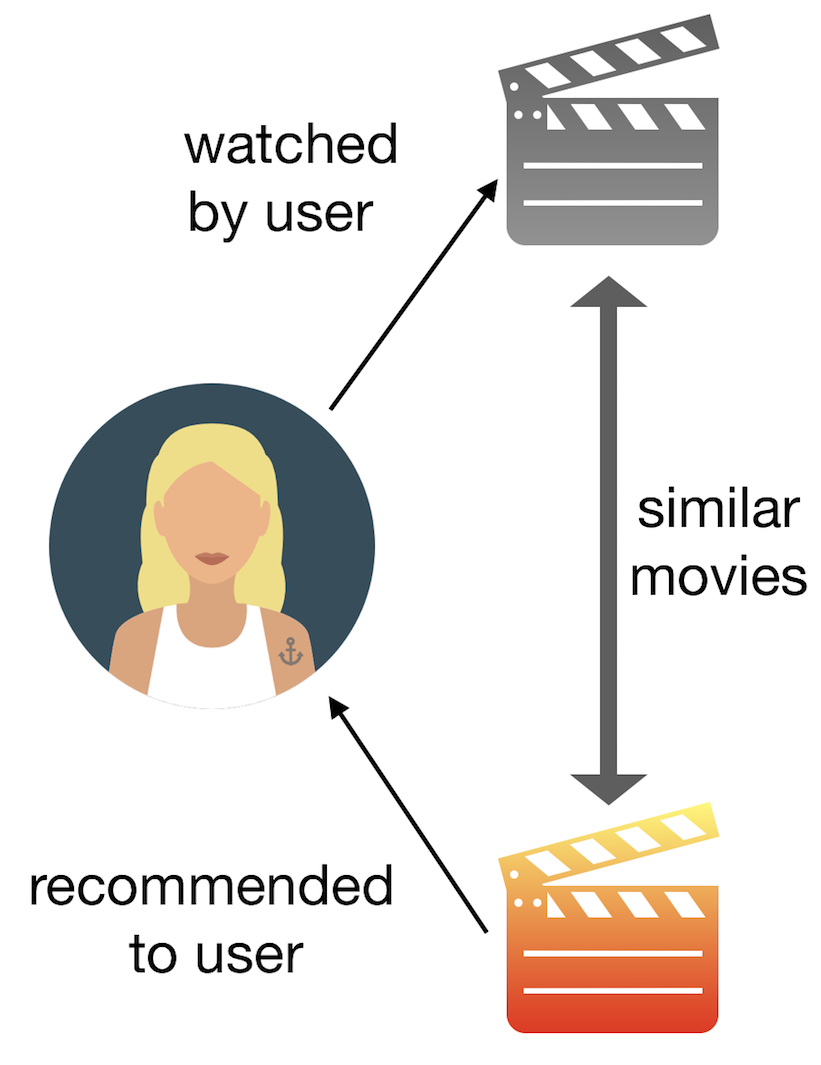
\includegraphics[height=4.5cm,width=3.5cm]{figures/Content-based.png}
		\end{figure}
	\newpage
	there are 2 approaches that claim to be “Content-based”:
	\begin{itemize}
	    \item Analysing Description of the Content Only
	    \item Building User Profile and Item Profile from User Rated Content
	\end{itemize}
\end{frame}

\subsection{Approach 1}
\begin{frame}[allowframebreaks, fragile]{Approach 1: Analysing the Description of Content Only}
    Based on my understanding, approach 1 is similar to item-based collaborative filtering. In short, the system will recommend anything similar to an item you like before.
    \begin{figure}
        \centering
        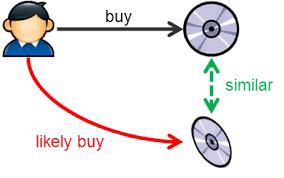
\includegraphics[scale=0.5]{figures/content-based-1.png}
    \end{figure}
    \newpage
    Usually the similarity will be derived from the description of the item and the concept of TF-IDF will be introduced. Then each item will be represented by a TF-IDF vector.\\
    \newline
    \textbf{Term Frequency-Inverse Document Frequency(TF-IDF)}
    \begin{enumerate}
        \item \textbf{Term Frequency:} Frequency of the word in the current document to the total number of words in the document.
        \begin{figure}
            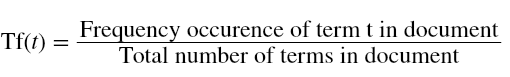
\includegraphics[scale=0.6]{figures/tf.PNG}
        \end{figure}
        \item \textbf{Inverse Document Frequency:} Total Number of Documents to the frequency occurrence of documents containing the word
        \begin{figure}
            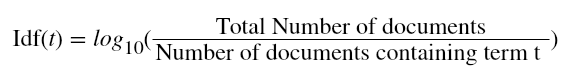
\includegraphics[scale=0.6]{figures/idtf.PNG}
        \end{figure}
    \end{enumerate}
    In the End, TF-IDF is a measure used to evaluate how important a word is to a document in a document corpus for example this table:
    \begin{figure}
        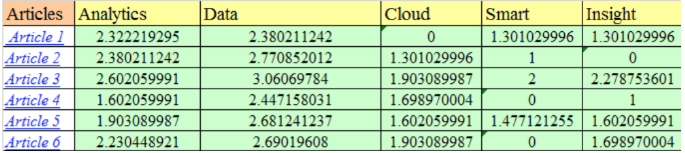
\includegraphics[scale=0.6]{figures/id-idtf.PNG}
    \end{figure}
    \textbf{Compare the Similarity of the item TF-IDF vector}
    To compute how similar the item vectors are, we will can use various methods such as:
    \begin{itemize}
        \item Cosine Similarity
        \item Euclidean Distance
        \item Peason’s Correlation
    \end{itemize}
\end{frame}

\subsection{Approach 2}
\begin{frame}{Approach 2: Building User Profile and Item Profile from User Rated Content}
it leverage description or attributes from items the user has interacted to recommend similar items. 
\begin{figure}
    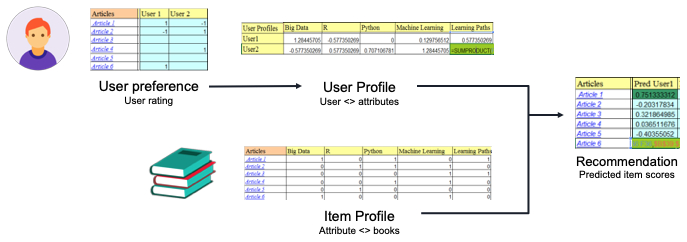
\includegraphics[scale=0.45]{figures/approach2.png}
\end{figure}
\end{frame}

\subsection{Pros and Cons}
\begin{frame}[allowframebreaks, fragile]{Pros and Cons}
    \textbf{Pros:}
    \begin{itemize}
        \item  \textbf{User independence:} Produce more reliable results with fewer users in the system.
        \item \textbf{Transparency:} Items are recommended on a feature-level basis.
        \item \textbf{No cold start:} New items can be suggested before being rated by a substantial number of users.
    \end{itemize}
    \textbf{Cons:}
    \begin{itemize}
        \item \textbf{Limited content analysis:} If the content doesn’t contain enough information to discriminate the items precisely, the recommendation itself risks being imprecise.
        \item \textbf{Over-specialization:} Content-based filtering provides a limited degree of novelty, since it has to match up the features of a user’s profile with available items.
        \item \textbf{New user:} when there’s not enough information to build a solid profile for a user, the recommendation could not be provided correctly.
    \end{itemize}
\end{frame}